%%% Preamble
\documentclass[paper=a4, fontsize=11pt]{scrartcl}	% Article class of KOMA-script with 11pt font and a4 format
\usepackage[T1]{fontenc}
\usepackage[utf8]{inputenc}
\usepackage[spanish]{babel}
\usepackage{fourier}
\usepackage{lmodern}

\usepackage[protrusion=true,expansion=true]{microtype} % Better typography
\usepackage{amsmath,amsfonts,amsthm} % Math packages
\usepackage[pdftex]{graphicx} % Enable pdflatex
\usepackage{url}

\usepackage{verbatim}

\usepackage{hyperref}
\hypersetup{%
  pdftitle={Operadores de manejo de bits en C},
  pdfauthor={Fernando CLADERA - Eduardo IRIARTE},
  pdfsubject={},
  bookmarksnumbered=true,
  bookmarksopen=true,
  bookmarksopenlevel=1,
  colorlinks=true,
  pdfstartview=Fit,
  pdfpagemode=UseOutlines,    % this is the option you were lookin for
  pdfpagelayout=TwoPageRight
}

%%% Custom sectioning (sectsty package)
\usepackage{sectsty} % Custom sectioning (see below)
\allsectionsfont{\centering \normalfont\scshape} % Change font of al section commands

%%% Custom headers/footers (fancyhdr package)
\usepackage{fancyhdr}
\pagestyle{fancyplain}
\fancyhead{} % No page header
\fancyfoot[L]{} % You may remove/edit this line
\fancyfoot[C]{} % Empty
\fancyfoot[R]{\thepage} % Pagenumbering
\renewcommand{\headrulewidth}{0pt} % Remove header underlines
\renewcommand{\footrulewidth}{0pt} % Remove footer underlines
\setlength{\headheight}{13.6pt}

%%% Better tables and matrices
\renewcommand*{\arraystretch}{2}

%%% Code is beautiful
\usepackage{minted}

%%% Equation and float numbering
\numberwithin{equation}{section} % Equationnumbering: section.eq#
\numberwithin{figure}{section} % Figurenumbering: section.fig#
\numberwithin{table}{section} % Tablenumbering: section.tab#

%%% Maketitle metadata
\newcommand{\horrule}[1]{\rule{\linewidth}{#1}} 	% Horizontal rule

\title{%
		%\vspace{-1in}
		\usefont{OT1}{bch}{b}{n}
		\normalfont \normalsize \textsc{Microcontroladores y Electrónica de
    Potencia} \\ [25pt]
		\horrule{0.5pt} \\[0.4cm]
		\huge Operadores de manejo de bits en C\\
		\horrule{2pt} \\[0.5cm]
}
\author{%
  \normalfont \normalsize
        Fernando CLADERA - Eduardo IRIARTE \\[-3pt]
        \normalsize
        Version 1 - \today
}
\date{}

%%% Begin document
\begin{document}
\maketitle

\section{Síntesis}

\begin{table}[h]
  \centering
  \begin{tabular} {l | l}
    \hline
    \textbf{Operación} & \textbf{Código en C} \\ \hline
    Poner a \verb|'1'| el bit \verb|n| de la variable \verb|var| & \verb!var |= (1<<n);! \\
    Poner a \verb|'0'| el bit \verb|n| de la variable \verb|var| & \verb!var &= ~(1<<n);! \\
    \emph{Toggle} del bit \verb|n| de la variable   \verb|var| & \verb!var ^= (1<<n);! \\
    Evaluar el bit \verb|n| de la variable   \verb|var| & \verb!var & (1<<n)! \\
    \hline
  \end{tabular}
\end{table}

\section{Introducción}

Los operadores de manejo de bits permiten realizar operaciones sobre los
bits de una variable.
Podemos clasificarlos en:
\begin{itemize}
  \item Operadores {bit a bit}
  \item Operadores de desplazamiento
\end{itemize}
En ciertos procesadores, las operaciones de manejo de bits están
soportadas directamente en el hardware. Por ejemplo, las instrucciones
\verb|SBI| y \verb|CLI| en AVR  (sólo para E/S) y \verb|BSF| y
\verb|BCF| en PIC\footnote{Estas permiten poner a \texttt{'1'}, a
\texttt{'0'} o evaluar el valor de un bit.}. En otros procesadores, esta
manipulación directa no está soportada, o solamente está permitida para
el área de E/S, por lo que se recurre a las técnicas que se explican a
continuación\footnote{La técnica leer/modificar/escribir tiene el
inconveniente de que esta secuencia podría ser interrumpida por otro
proceso que afecte la misma variable.  Esto no pasa en las instrucciones
de manipulación directa como las antedichas (que son atómicas). Las de
evaluación de bit no tienen este problema.}.

\section{Operadores bit a bit}

Permiten efectuar operaciones lógicas (AND, OR, NOT, XOR) sobre los bits
de una variable. Son particularmente útiles en la programación de
microcontroladores, donde deben realizarse operaciones en bits
específicos de un registro.

\begin{table}[h]
  \centering
  \small
  \begin{tabular}{l | l | l | l}
    \hline
    \textbf{Nombre} & \textbf{Operador} & \textbf{Ejemplo en C} & \textbf{Representación en binario} \\ \hline
    AND & Ampersand & \verb!uint8_t a = 0xF1 & 0x0F;! & \verb!"11110001" & "00001111"! \\
    & \verb!&! & \verb!// a = 0x01! & \verb!= "00000001"! \\ \hline
    OR & Pipe & \verb!uint8_t a = 0xF1 | 0x0F;! & \verb!"11110001" | "00001111"!  \\
    & \verb!|! & \verb!// a = 0xFF! & \verb!= "11111111"! \\ \hline
    XOR & Caret & \verb!uint8_t a = 0xF1 ^ 0x0F;!  & \verb!"11110001" ^ "00001111"!  \\
    & \verb!^! & \verb!// a = 0xFE! & \verb!= "11111110"! \\ \hline
    NOT  & Tilde & \verb!uint8_t a = ~0xF1;! & \verb!~"11110001"! \\
    & \verb!~! & \verb!// a = 0x0E! & \verb!= "00001110"! \\ \hline
  \end{tabular}
\end{table}
\textbf{Nota:} \verb|uint8_t| es una variable de tipo \emph{unsigned} de
8 bits. Ver \verb|stdint.h|.

\section{Operadores de desplazamiento}

Tal como su nombre lo indica, permiten realizar desplazamientos de bits.
Por ejemplo, si disponemos del valor \verb|"00010110"| y realizamos un
desplazamiento a la izquierda, obtenemos el valor \verb|"00101100"|. Observamos
que en este caso, se {pierde} un bit a la izquierda y se
{agrega} un nuevo bit \verb|'0'| a la derecha.

El desplazamiento de bits a izquierda y derecha, para variables de tipo
\textbf{\emph{unsigned}}, puede entenderse como una multiplicación y una división entera
respectivamente. Los bits agregados luego del desplazamiento son
\verb!'0'!.

\begin{itemize}
  \item \verb!a << n = a * 2^n!

    Ej: \verb!5 << 2 = "00000101" << 2 = "00010100" = 20!

  \item \verb!a >> n = a / 2^n!

    Ej: \verb!23 >> 2 = "00010111" = "00000101" = 5!
\end{itemize}

\begin{table}[h]
  \centering
  \small
  \begin{tabular}{l | l | l | l}
    \hline
    \textbf{Nombre} & \textbf{Operador} & \textbf{Ejemplo en C} & \textbf{Representación en binario} \\ \hline
    Desp. a la izq. & \verb!<<! & \verb!uint8_t a = 0x01 << 4;! & \verb!"00000001" << 4! \\
    & & \verb!// a = 0x10! &\verb!= "00010000"! \\ \hline
    Desp. a la der. & \verb!>>! & \verb!uint8_t a = 0x10 >> 4;!  & \verb!"00010000" >> 4!\\
    & & \verb!// a = 0x01! &  \verb! = "00000001"! \\ \hline
  \end{tabular}
\end{table}

El desplazamiento de bits en variables de tipo \textbf{\emph{signed}} presenta el
comportamiento siguiente:
\begin{itemize}
  \item El \textbf{desplazamiento a la derecha} está definido por la
    implementación del compilador. Los bits agregados luego del
    desplazamiento pueden ser del valor del
    bit más significativo (MSB), o pueden ser \verb!'0'!.
  \item El \textbf{desplazamiento a la izquierda} {\color{red}tiene un
    comportamiento indefinido}.
\end{itemize}

Como conclusión, podemos decir que \textbf{no es una buena idea}
realizar desplazamientos de bits en variables \emph{signed}, salvo que
se conozca con precisión las características de la plataforma y el
compilador.

\section{Operaciones sobre registros de un microcontrolador}

Si se desea configurar el Timer 0 del microcontrolador ATmega328 (AVR
8 - Arduino Uno/Nano), es necesario modificar el registro \verb|TCCR0A|. De la hoja de datos del
microcontrolador observamos los diferentes campos del registro:

\begin{figure}[h]
  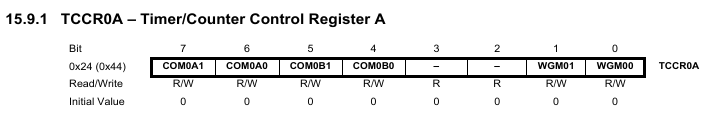
\includegraphics[width=\textwidth]{ATMEGA-timer.png}
\end{figure}

Se observa que mediante este registro pueden modificarse 3 parámetros
del Timer 0 (\emph{la función de estos parámetros no es importante en este
momento}):
\begin{itemize}
  \item \verb|COM0Ax| (bits 7:6) - Compare Match Output A Mode
  \item \verb|COM0Bx| (bits 5:4) - Compare Match Output B Mode
  \item \verb|WGM0x| (bits 1:0) - Waveform Generation Mode
\end{itemize}

\subsection{Ejemplo 1 - Escritura de registros con AND y OR}

Se plantea el problema de modificar los bits de \verb|COM0Bx|, sin
modificar el resto de los bits del registro. Específicamente, se
requiere escribir un \verb|'1'| en el bit 5 (\verb|COM0B1|) y un
\verb|'0'| en el bit 4 (\verb|COM0B0|).  Se presenta el siguiente código
de ejemplo, utilizando operadores {bit a bit}:

\begin{minted}[mathescape,
               numbersep=5pt,
               gobble=0,
               frame=lines,
               framesep=2mm,fontsize=\small]{c}
TCCR0A &= 0xEF  // Mediante AND con el valor "11101111" (máscara)
                // se coloca a ‘0’ el bit 4
TCCR0A |= 0x20  // Mediante OR con "00100000" se coloca a ‘1’ el bit número 5
                // los otros bits permanecen en el estado anterior
\end{minted}

El código propuesto, si bien cumple con el objetivo de la consigna, es
complejo debido a la necesidad de especificar los valores hexadecimales de
las máscaras.

\subsection{Ejemplo 2 - Escritura de registros con desplazamiento de bits}

Podemos utilizar los desplazamientos de bits para analizar el ejemplo
anterior:

\begin{minted}[mathescape,
               numbersep=5pt,
               gobble=0,
               frame=lines,
               framesep=2mm,fontsize=\small]{c}
TCCR0A &= ~(1<<4);  // Se coloca a '0' el bit 4
TCCR0A |= 1<<5;     // Se coloca a '1' el bit número 5
\end{minted}

Observamos que 
\begin{itemize}
    \item \verb!~(1<<4) = 0xEF!
    \item \verb!1<<5 = 0x20!
\end{itemize}
No obstante, este ejemplo no es fácilmente legible. Es necesario contar
con la hoja de datos del microcontrolador para saber qué campos están
siendo modificados en \verb|TCCR0A|.

\subsection{Ejemplo 3 - Escritura de registros mediante headers}

Generalmente, las cabeceras (\emph{headers}, .h) que definen los
registros de un microcontrolador especifican los diferentes
campos. Para el ATmega 328, la
cabecera que define el microcontrolador establece las siguientes
constantes:

\begin{minted}[mathescape,
               numbersep=5pt,
               gobble=0,
               frame=lines,
               framesep=2mm,fontsize=\small]{c}
#define WGM00 0
#define WGM01 1
#define COM0B0 4
#define COM0B1 5
#define COM0A0 6
#define COM0A1 7
\end{minted}
Por consiguiente, podemos reescribir el ejemplo anterior como
\begin{minted}[mathescape,
               numbersep=5pt,
               gobble=0,
               frame=lines,
               framesep=2mm,fontsize=\small]{c}
TCCR0A &= ~(1<<COM0B0); // Colocamos a '0' el bit correspondiente a COM0B0
TCCR0A |= 1<<COM0B1;    // Colocamos a '1' el bit correspondiente a COM0B1
\end{minted}

En este código es fácil ver la operación sobre los registros,
y analizar el resultado final de \verb|COM0Bx| en \verb|TCCR0A|. Por
consiguiente, \textbf{se trata de la respuesta más adecuada para el
problema propuesto}.

\subsection{Ejemplo 4 - Toggle de bits de un registro}

Utilizando el operador XOR podemos cambiar el estado de un bit
(\emph{toggle}). Por ejemplo, si deseamos cambiar el estado del bit
\verb|COM0B1| de \verb|TCCR0A|, podemos escribir:

\begin{minted}[mathescape,
               numbersep=5pt,
               gobble=0,
               frame=lines,
               framesep=2mm,fontsize=\small]{c}
TCCR0A ^= (1<<COM0B1);    // Toggle de bit COM0B1
\end{minted}

\subsection{Ejemplo 5 - Evaluación del estado de un bit de un registro}

Finalmente, si deseamos evaluar el estado de un bit, podemos
hacer un simple AND {bit a bit}. Por ejemplo, para evaluar el
estado de \verb|COM0B0| de \verb|TCCR0A|, podemos escribir

\begin{minted}[mathescape,
               numbersep=5pt,
               gobble=0,
               frame=lines,
               framesep=2mm,fontsize=\small]{c}
if (TCCR0A & (1<<COM0B0)) {
  // Detectamos que COM0B0 está en '1'
  printf("TCCR0A - COM0B0: 1\n");
} else {
  // Detectamos que COM0B0 está en '0'
  printf("TCCR0A - COM0B0: 0\n");
}
\end{minted}

\section{Links útiles}

{
  \footnotesize
\url{http://www.catonmat.net/blog/low-level-bit-hacks-you-absolutely-must-know/}

\url{http://graphics.stanford.edu/~seander/bithacks.html}
}
%%% End document
\end{document}
